\documentclass[a5paper,headsepline,titlepage,11pt,nnormalheadings,DIVcalc]{scrbook}
\usepackage[a5paper,backref]{hyperref}
\usepackage[papersize={148.5mm,210mm},twoside,bindingoffset=0.5cm,hmargin={1cm,1cm},
				vmargin={1.5cm,1.5cm},footskip=0.65cm,driver=dvipdfm]{geometry}
\usepackage{palatino}
\usepackage{microtype}
\usepackage{graphicx}
\usepackage{wrapfig}
\usepackage[bahasa]{babel}
\usepackage{fancyhdr}
\usepackage{pstricks}
%\setlength{\voffset}{0.5in}
%\setlength{\oddsidemargin}{28pt}
%\setlength{\evensidemargin}{0pt}
\renewcommand{\footrulewidth}{0.5pt}
\lhead[\fancyplain{}{\thepage}]%
      {\fancyplain{}{\rightmark}}
\rhead[\fancyplain{}{\leftmark}]%
      {\fancyplain{}{\thepage}}
\pagestyle{fancy}
\lfoot[\emph{Ziarah Goa Maria Jatingsih}]{}
\rfoot[]{\emph{Lingkungan St Theresia Maguwo}}
\cfoot{}

\newcommand{\BU}[1]{\begin{itemize} \item[U:] #1 \end{itemize}}
\newcommand{\BI}[1]{\begin{itemize} \item[I:] #1 \end{itemize}}
\newcommand{\BP}[1]{\begin{itemize} \item[P:] #1 \end{itemize}}
\newcommand{\kamiMenyembah}{\BP{ Kami menyembah Dikau ya Tuhan dan bersyukur\\kepadaMu.}
\BU{ Sebab dengan salib suciMu, Engkau telah menebus dunia.}
}
\newcommand{\kasihanilahKami}{\BP{Demi sengsara Yesus yang pedih \ldots,}
\BU{tunjukkanlah belas kasih-Mu kepada kami dan seluruh dunia.}}
\def\hening{\par \textit{(Hening sejenak)}}


\title{Jalan Salib\\Berdasarkan Refleksi Yesus}
\author{Ziarah Taman Doa Goa Maria Pereng\\Lingkungan St. Petrus Maguwo}
\date{21 Mei 2016}
\hyphenation{sa-u-da-ra-ku}
\hyphenation{ke-ri-ngat}
\hyphenation{je-ri-tan}
\hyphenation{hu-bung-an}
\hyphenation{me-nya-dari}
\hyphenation{Eng-kau}
\hyphenation{ke-sa-lah-an}
\hyphenation{ba-gai-ma-na}
\hyphenation{Tu-han}
\hyphenation{di-per-ca-ya-kan}
\hyphenation{men-ja-uh-kan}
\hyphenation{bu-kan-lah}
\hyphenation{per-sa-tu-kan-lah}
\hyphenation{ma-khluk}
\hyphenation{Sem-buh-kan-lah}
\hyphenation{ja-lan}
\hyphenation{mem-bu-tuh-kan}
\hyphenation{be-ri-kan-lah}
\hyphenation{me-ra-sa-kan}
\hyphenation{te-man-ilah}
\hyphenation{mem-bi-ngung-kan}
\hyphenation{di-ka-gum-i}
\hyphenation{ta-ngis-an-Mu}
\hyphenation{mi-lik-ilah}


\begin{document}
%\maketitle
\thispagestyle{empty}
\newsavebox\IBox
\sbox\IBox{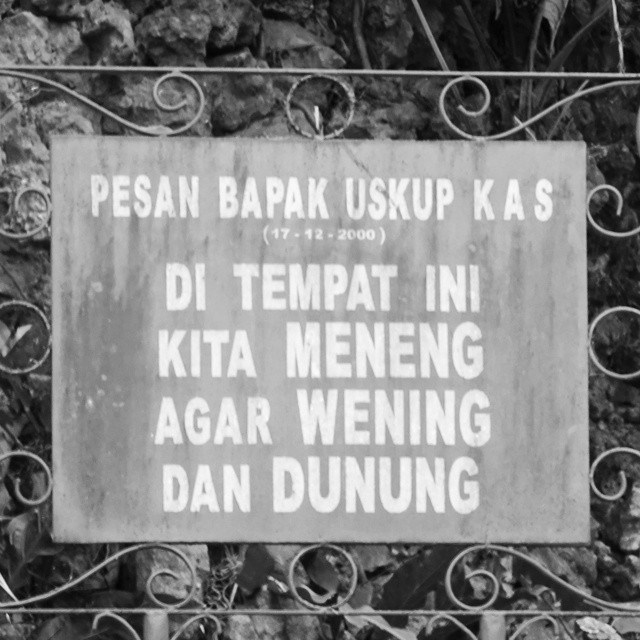
\includegraphics[scale=0.5]{jatiningsih2.jpg}}
% set up the picture environment
\psset{unit=1in}
\begin{center}
\begin{pspicture}(4in,6in)
% set up the fonts we use
\DeclareFixedFont{\PT}{T1}{ppl}{b}{it}{0.25in}
\DeclareFixedFont{\PTsmall}{T1}{ppl}{b}{it}{0.2in}
\DeclareFixedFont{\PTsmallest}{T1}{ppl}{b}{it}{0.15in}
\DeclareFixedFont{\PTtext}{T1}{ppl}{b}{it}{11pt}
\DeclareFixedFont{\Logo}{T1}{pbk}{m}{n}{0.15in}
% place the front cover picture
\rput[cb](2,2.5){\usebox\IBox}
% put the text on the front cover
\rput[cb](2,5.5){\PT {JALAN SALIB}}
\rput[cb](2,5.125){\PT {Ziarah Goa Maria Jatiningsih}}
\rput[cb](2,4.85){\PTsmall {Sendangarum Moyudan Sleman}}
\rput[cb](2,-0.05){\PTsmallest {Lingkungan St Theresia Maguwo}}
\rput[cb](2,-0.2){\PTsmallest {21 Mei 2016}}

%\rput[cb](3,-1){\PTsmallest {\namagereja}} 

\end{pspicture}
\end{center}
\newpage
\subsection*{PEMBUKAAN}
\begin{itemize}
\item[~] Lagu Pembukaan
\item[~] SengsaraMu, O Yesus - MB 279
\item[1.] \it{
SengsaraMu, O Yesus, akibat dosaku\\
Kau dihina disiksa, dibunuh rakyatMu\\
Gembala yang utama mengorbankan diri\\
Supaya kumpulanMu, luput dari mati 
}
\item[3.] \it{
Allah yang maharahim, ampunilah dosa\\
demi cinta PutraMu, dan kurban salibNya\\
Berilah kurniaMu, agar teladanNya\\
mengorbankan hatiku, dengan cinta mesra
}
\end{itemize}

\BP{Dalam nama Bapa, dan Putra, dan Roh Kudus. }
\BU{Amin}
 
\BP{Berikanlah dirimu dipeluk oleh kerinduan-Ku yang paling bernyala-nyala agar segenap jiwa-jiwa datang dan memurnikan diri mereka dalam air tobat, dan agar kepercayaan, bukan takut, merasuki mereka, sebab Aku adalah Tuhan Yang Maharahim dan Aku senantiasa siap menerima mereka dalam Hati-Ku.

Apabila engkau melakukan apa yang Aku minta, Aku dekat denganmu. Ketaatanmu akan memuaskan dahaga dahsyat yang mengeringkan bibir-Ku di Salib.

Aku akan menghadirkan DiriKu setiap kali engkau merenungkan Passio-Ku dengan kasih. Aku akan mengijinkanmu untuk tinggal bersatu dengan-Ku dalam sengsara yang Aku derita di Getsemani ketika Aku mengenali dosa-dosa segenap umat manusia.

Renungkanlah segala sesuatu yang harus Aku alami agar dapat menyelamatkan manusia, agar dapat bertahta dalam hatinya, agar memungkinkannya masuk ke dalam Kerajaan Bapa-Ku.

Marilah sekarang kita merenungkan Passio-Ku \dots yang akan terus mendatangkan kemuliaan bagi Bapa dan kekudusan bagi jiwa-jiwa.}

\BU{Oh Yesus, kami berdiri dalam penderitaan di kaki salibMu: kami sendiri telah membantu menegakkannya dengan dosa-dosa kami! Kebaikanmu yang tidak menawarkan perlawanan, dan membiarkannya sendiri untuk disalibkan, adalah sebuah misteri di luar genggaman kami; ia menyisakan kegelisahan yang amat mendalam. Tuhan, Engkau datang ke dunia bagi kami, untuk mencari dan menunjukkan kepada kami rangkulan penuh kasih dari Bapa:
 Luk 15:20 rangkulan yang amat kami nantikan! Engkau adalah Wajah yang sejati dari keindahan dan dari belas kasih: itulah mengapa Engkau ingin menyelamatkan kami! Dalam diri kami ada penuh keegoisan: datanglah kepada kami dengan kasihMu yang membebaskan! Dalam diri kami ada keseombongan dan kebencian: datanglah kepada kami dengan kelembutan dan kerendahan hatiMu! Tuhan, kami adalah pendosa yang perlu diselamatkan: kami adalah anak pemboros yang perlu kembali! Tuhan, berikanlah kepada kami hadiah air mata! Sehingga kami boleh menemukan sekali lagi kebebasan dan kehidupan, kedamaian denganMu, dan kegembiraan di dalam Engkau, Amin.} 

\begin{itemize}\item[~]\textit{
\setlength{\tabcolsep}{0pt}
\begin{tabular}{cccccccccc}
&1&2&3&2&3&5&4&3&.\\
1.&Ma-&ri-&lah&ki-&ta&re-&nung-&kan\\
&3&2&1&\d{7}&\d{6}&\d{7}&\d{6}&\d{5}&.\\
&Ye-&sus~~&yang~~&men-&ja-&di&kur-&ban\\
&2&1&2&3&2&1&1&.    //\\
&kar'-&na&cin-&ta&ka-&sih-&nya
\end{tabular}}
\end{itemize}

\begin{wrapfigure}[0]{r}{2cm}
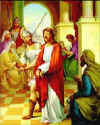
\includegraphics[width=2cm]{jalansalib_files/01_small.jpg}
\end{wrapfigure}
\subsection*{Perhentian I \\
YESUS DI JATUHI HUKUMAN MATI}

\kamiMenyembah
\BP{Yesus dijatuhi hukuman mati
Meski tidak bersalah, Yesus tetap dijatuhi hukuman mati. Ia dianggap sebagai orang yang telah melanggar aturan kemapanan. Padahal yang diwartakan-Nya adalah kebenaran, kasih dan kebahagiaan. Aneh memang, manusia lebih senang hidup dalam kegelapan, kekacauan dan kesenangan sia-sia. Yesus tetap diam.  Sikap diam-Nya bukan berarti membiarkan ketidakadilan merajalela. Ia diam sebagai wujud ketaatan total-Nya kepada kehendak Bapa. Demi manusia, Ia rela menanggung hukuman yang tidak seharusnya Ia jalani. Dengan diam, Ia hendak menunjukkan bahwa kasih adalah kekuatan yang tak terkalahkan oleh kejahatan, iri dengki, dan balas dendam. Ia rela menerima itu semua karena cinta-Nya pada manusia tak terbatas. Ia menunjukkan bahwa diam bukan berarti mati. Diam dan menerima realitas penderitaan adalah jalan hidup yang telah dipilih-Nya demi perutusan yang amat agung, yakni menebus dosa manusia. Beranikah kita membalas kasih terhadap orang-orang yang telah menyakiti kita? Atau kita justru menyakiti saudara kita yang telah mengasihi kita dengan tulus?
\hening
}

\BU{Akupun menghakimi Engkau ya Yesus,\\ dalam diri sesamaku.\\ Ampunilah aku.\\
Tuhan kasihanilah kami (2X)}
 
\large\begin{itemize}\item[~]\it{Bapa Kami - Salam Maria}\end{itemize}\normalsize

\kasihanilahKami

\begin{itemize}
\item[2.] \it{Sri Yesus Penebus kami,\\ 
	dijatuhi hukum mati,\\ 
	agar umatNya hidup}
\end{itemize}



\begin{wrapfigure}[0]{r}{2cm}
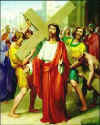
\includegraphics[width=2cm]{jalansalib_files/02_small.jpg}
\end{wrapfigure}
\subsection*{Perhentian II\\
YESUS MEMANGGUL SALIBNYA}


\kamiMenyembah
\BP{Salib berat diterima-Nya. Dengan tegar, Ia memanggul salib yang akan menjadi tempat-Nya bergantung dan disiksa. Yesus bukan seorang pengecut yang lari dari penderitaan yang mesti dihadapi-Nya. Meski berat, Ia tetap memanggul salib itu dengan mantap. Sorot mata-Nya lurus memandang ke depan. Lalu dengan tertatih Ia mulai berjalan. Ia memanggul penderitaan dan ketidaksempurnaan manusia. Apakah aku berani mengikuti Yesus yang penuh dedikasi dalam menjalankan perintah Bapa-Nya? Atau justru aku lari bak seorang pengecut yang tak berani bertanggung jawab atas segala resiko dari perjuanganku sebagai anak-anak-Nya?

\hening
}

\BU{Akupun menaruh berbagai beban di pundak sesamaku\\ padahal hidup mereka sendiri sudah susah.\\ Ampunilah aku ya Yesus\\ 
Tuhan kasihanilah kami (2X)}



\large\begin{itemize}\item[~]\it{Bapa Kami - Salam Maria}\end{itemize}\normalsize
\kasihanilahKami

\begin{itemize}
\item[3.] \it{Salib berat dipanggulNya,\\ 
	agar kita ikutiNya,\\ 
	memikul salib kita}
\end{itemize}

\begin{wrapfigure}[0]{r}{2cm}
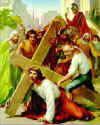
\includegraphics[width=2cm]{jalansalib_files/03_small.jpg}
\end{wrapfigure}
\subsection*{Perhentian III\\
YESUS JATUH PERTAMA KALINYA DIBAWAH\\SALIBNYA}

\kamiMenyembah
\BP{Kekuatan fisik Yesus pun terbatas. Setelah didera dan memanggul salib berat, kekuatan Yesus berkurang amat drastis. Ia jatuh tertimpa salib untuk pertama kalinya. Luka baru muncul di beberapa bagian tubuh-Nya. Bukan bantuan yang Ia terima tetapi justru pukulan dan cambukan dari para serdadu. Dengan tubuh berlumur darah, Yesus bangkit lagi dan meneruskan perjalanan. Yesus adalah raja, tetapi justru karena kesediaan-Nya untuk direndahkan dan tersungkur di bawah salib, Ia telah menunjukkan bahwa keagungan terletak pada kesediaan untuk bangkit dan kembali berjuang. Apakah kita sering merasa sempurna dan tak pernah jatuh hingga tak perlu bangkit? Atau justru kita senang dan membiarkan begitu saja ketika melihat teman kita sedang terjatuh?
(hening sejenak)
}

\BU{Akupun tidak menolong sesamaku yang susah hidupnya\\ agar ia bangkit. \\Berbelaskasihlah padaku ya Yesus\\
 Tuhan kasihanilah kami (2X)
}

\large\begin{itemize}\item[~]\it{Bapa Kami - Salam Maria}\end{itemize}\normalsize
\kasihanilahKami

\begin{itemize}
\item[4.] \it{Sri Yesus tolonglah kami, \\
	bila kami jatuh lagi,\\ 
	tertindih salib berat.}
\end{itemize}

\begin{wrapfigure}[0]{r}{2cm}
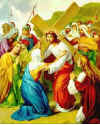
\includegraphics[width=2cm]{jalansalib_files/04_small.jpg}
\end{wrapfigure}
\subsection*{Perhentian IV\\
YESUS BERJUMPA DENGAN BUNDANYA}

\kamiMenyembah
\BP{Di tengah perjalanan, Yesus berjumpa dengan ibu-Nya.  Yesus mencintai manusia sampai sakit, bahkan sampai wafat di salib. Ia tahu bahwa Bunda Maria pun mengalami hal yang sama. Bunda Maria telah mencintai Putranya hingga sakit. Hati Bunda Maria merasakan pedih yang mendalam saat menyaksikan putra yang amat dikasihinya itu menderita. Apakah kita berani mencintai hingga sakit seperti Yesus dan Bunda Maria ? Atau kita justru membuat orang lain sakit dan menangis karena kita hanya memikirkan kesenangan pribadi?
\hening
}

\BU{Aku pun menyebabkan orang lain menangis,\\ padahal mereka mencintai aku.\\ Yesus hiburlah mereka\\
Tuhan kasihanilah kami (2X)
}

\large\begin{itemize}\item[~]\it{Bapa Kami - Salam Maria}\end{itemize}\normalsize
\kasihanilahKami

\begin{itemize}
\item[5.] \it{Maria selalu setia,\\ 
	pada Sang Kristus Putranya,\\ 
	dalam suka dan duka.}
\end{itemize}

\begin{wrapfigure}[0]{r}{2cm}
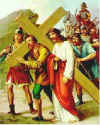
\includegraphics[width=2cm]{jalansalib_files/05_small.jpg}
\end{wrapfigure}
\subsection*{Perhentian V\\
SIMON KIRENE MEMBANTU YESUS\\MEMANGGUL SALIBNYA}

\kamiMenyembah
\BP{Yesus terlihat semakin lemah. Lalu muncul seorang yang mau membantu-Nya memanggul salib. Yesus memberkati Simon karena kesediaannya menolong orang yang menderita. Apakah kita mau menolong orang yang menderita dengan tulus hati? Atau kita takut mendapatkan penderitaan yang sama ketika kita hendak menolong orang itu?
\hening
}

\BU{Aku tidak selalu membantu orang yang memerlukan pertolonganku.\\ Yesus, terimalah penyesalanku!\\
Tuhan kasihanilah kami (2X)
}


\large\begin{itemize}\item[~]\it{Bapa Kami - Salam Maria}\end{itemize}\normalsize
\kasihanilahKami

\begin{itemize}
\item[6.] \it{Cinta bakti pada Tuhan,\\ 
	hanya dapat dibuktikan, \\
	dengan saling mengabdi.}
\end{itemize}

\begin{wrapfigure}[0]{r}{2cm}
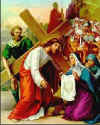
\includegraphics[width=2cm]{jalansalib_files/06_small.jpg}
\end{wrapfigure}
\subsection*{Perhentian VI\\
VERONIKA MENGUSAP WAJAH YESUS}

\kamiMenyembah

\BP{Melihat wajah Yesus yang berlumuran keringat, darah dan debu, Veronika lari kepada Yesus dan mengusap wajah-Nya. Meski amat sederhana, Veronika telah mewujudkan betapa Ia mencintai Yesus. Cinta tak sekedar kata-kata. Cinta adalah sebuah perjuangan agar orang yang dicintai memperoleh kebahagiaan dan keselamatan. Meski untuk itu, dirinya sendiri terancam bahaya. Apakah kita berani mencintai Tuhan dan sesama seperti Veronika yang sederhana dan tulus?
\hening
}

\BU{Betapa seringnya aku lari menghindar menghadapi sesama,\\ padahal aku dapat meringankan bebannya.\\
Tuhan kasihanilah kami (2X)
}


\large\begin{itemize}\item[~]\it{Bapa Kami - Salam Maria}\end{itemize}\normalsize
\kasihanilahKami
 
\begin{itemize}
\item[7.] \it{
Lipuran yang meringankan,\\ 
	duka orang yang tertekan,\\ 
	menghibur Kristus juga.
}
\end{itemize}

\begin{wrapfigure}[0]{r}{2cm}
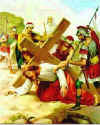
\includegraphics[width=2cm]{jalansalib_files/07_small.jpg}
\end{wrapfigure}

\subsection*{Perhentian VII\\
YESUS JATUH UNTUK KEDUA KALINYA}

\kamiMenyembah

\BP{Yesus kembali jatuh di bawah salib. Kali ini lebih parah. Namun tak ada seorang pun yang membantu-Nya. Apakah kita termasuk orang-orang yang tak mau membantu Yesus untuk bangkit berdiri? Apa yang aku lakukan ketika melihat teman-temanku menderita? Apakah diam saja? Bisa jadi demikian, namun yang jelas, Yesus tinggal di dalam diri sesama kita, siapapun dia.
\hening
}

\BU{Tidak jarang aku berpura-pura tidak melihat penderitaan orang lain.\\ Yesus, berbelaskasihlah padaku!\\
Tuhan kasihanilah kami (2X)
}


\large\begin{itemize}\item[~]\it{Bapa Kami - Salam Maria}\end{itemize}\normalsize
\kasihanilahKami

\begin{itemize}
\item[8.] \it{Bilamana kami lemah,\\
	 jatuh tercampak di tanah,\\ 
	tegakkan kami lagi.}
\end{itemize}

\begin{wrapfigure}[0]{r}{2cm}
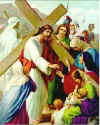
\includegraphics[width=2cm]{jalansalib_files/08_small.jpg}
\end{wrapfigure}
\subsection*{Perhentian VIII\\
YESUS MENGHIBUR WANITA-WANITA YANG\\MENANGIS}
\kamiMenyembah

\BP{Amat besar cinta wanita-wanita Yerusalem itu pada Yesus. Mereka menangisi Yesus yang menderita. Mereka turut merasakan bagaimana sakitnya Yesus. Mereka turut merasakan betapa kesepiannya Yesus. Mereka turut merasakan betapa perihnya hati Yesus. Mereka mampu berbela rasa terhadap penderitaan orang lain.
\hening 
}

\BU{Aku lebih menangisi diriku sendiri\\ daripada kejahatan yang melukai Engkau ya Yesus,\\ dan yang membawa manusia ke dalam kebinasaan.\\ Ampunilah aku
Tuhan kasihanilah kami (2X)
}

\large\begin{itemize}\item[~]\it{Bapa Kami - Salam Maria}\end{itemize}\normalsize
\kasihanilahKami

\begin{itemize}
\item[9.] \it{Tobatkanlah jiwa kami, \\
	arahkanlah sikap hati,\\ 
	pada cinta sejati. 
}
\end{itemize}

\begin{wrapfigure}[0]{r}{2cm}
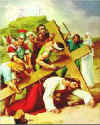
\includegraphics[width=2cm]{jalansalib_files/09_small.jpg}
\end{wrapfigure}
\subsection*{Perhentian IX\\
YESUS JATUH KETIGA KALINYA DIBAWAH SALIB}

\kamiMenyembah

\BP{Peristiwa jatuh selalu sakit dan menyisakan luka. Namun, jatuh bukanlah akhir dari perjuangan. Peristiwa jatuh justru semakin membuat manusia sadar bahwa tanpa rahmat Allah, manusia tak mampu melanjutkan kembali perjalanannya menuju ke Golgota untuk dipersatukan dengan Yesus.
\hening
}

\BU{Berilah aku rahmat, ya Yesus,\\ untuk mengalami Golgotaku bersama-Mu\\ dan didalam diri-Mu\\
Tuhan kasihanilah kami (2X)
}

\large\begin{itemize}\item[~]\it{Bapa Kami - Salam Maria}\end{itemize}\normalsize
\kasihanilahKami

\begin{itemize}
\item[10.] \it{Bila hatiku gelisah,\\
	Kar’na dosa atau susah,\\
	ulurkanlah tangan-Mu.}
\end{itemize}

\begin{wrapfigure}[0]{r}{2cm}
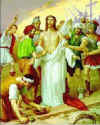
\includegraphics[width=2cm]{jalansalib_files/10_small.jpg}
\end{wrapfigure}
\subsection*{Perhentian X\\
PAKAIAN YESUS DITANGGALKAN}

\kamiMenyembah

\BP{Raja duniawi selalu berbangga dengan jubahnya yang indah, pakaiannya yang gemerlap, dan asesorisnya yang mewah. Namun Yesus, Raja segala raja justru ditinggikan dengan melepaskan seluruh pakaian-Nya. Sebab hanya dengan telanjang, orang benar-benar tulus, jujur, tanpa topeng, lepas bebas, dan suci. Yesus tidak membanggakan hak milik duniawi namun Ia menunjukkan keagungan-Nya dalam melepaskan segala sesuatu yang dianggap mulia oleh dunia, entah itu kuasa, kehormatan, harta, gengsi, dan kenikmatan.
\hening
}

\BU{Tutupilah ya Yesus ketelanjanganku dengan mantel kerahiman-Mu,\\ pada saat aku nanti menghadapi Bapa yang Mahaadil\\
Tuhan kasihanilah kami (2X)
}

\large\begin{itemize}\item[~]\it{Bapa Kami - Salam Maria}\end{itemize}\normalsize
\kasihanilahKami

\begin{itemize}
\item[11.] \it{PakaianMu dibagikan,\\
	jubah utuh diundikan,\\
	martabatMu dihina.}
\end{itemize}

\begin{wrapfigure}[0]{r}{2cm}
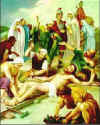
\includegraphics[width=2cm]{jalansalib_files/11_small.jpg}
\end{wrapfigure}
\subsection*{Perhentian XI\\
YESUS DIPAKU DI KAYU SALIB}

\kamiMenyembah

\BP{Saliblah yang menjadi tahta Yesus dan luka-luka di tangan serta kaki-Nya menjadi hiasan yang paling gemerlap.Begitu besarnya cinta Yesus pada kita. Hingga rela tergantung di kayu hina dengan penderitaan yang tiada tara. Tangan-Nya yang terentang terpaku di kayu salib adalah wujud keterbukaan hati-Nya untuk merengkuh dunia agar mereka semua terselamatkan.
\hening
}

\BU{Dalam luka-luka-Mu ya Yesus,\\ sembunyikanlah aku,\\ tunjukkanlah belaskasih-Mu padaku.\\
Tuhan kasihanilah kami (2X)
}

\large\begin{itemize}\item[~]\it{Bapa Kami - Salam Maria}\end{itemize}\normalsize
\kasihanilahKami

\begin{itemize}
\item[12.] \it{Dari salibMu Kaulihat,\\
	tak terbilang yang menghujat,\\
	berapakah yang setia?}
\end{itemize}


\begin{wrapfigure}[0]{r}{2cm}
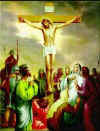
\includegraphics[width=2cm]{jalansalib_files/12_small.jpg}
\end{wrapfigure}
\subsection*{Perhentian XII\\
YESUS WAFAT DI SALIB}

\kamiMenyembah

\BP{\textit{Merenungkan wafat Yesus dengan meditasi singkat}}

\BU{Terimalah aku ya Yesus\\ sebagaimana Engkau telah menerima penyamun yang baik,\\ tetapi bangkitkanlah dalam diriku harapan dan rasa syukur kepada-Mu\\
Tuhan kasihanilah kami (2X)}

\large\begin{itemize}\item[~]\it{Bapa Kami - Salam Maria}\end{itemize}\normalsize
\kasihanilahKami

\begin{itemize}
\item[13.] \it{Benih yang mati hasilkan,\\
	buah yang berkelimpahan,\\
	wafatMu: sumber hidup.}
\end{itemize}

\begin{wrapfigure}[0]{r}{2cm}
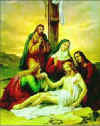
\includegraphics[width=2cm]{jalansalib_files/13_small.jpg}
\end{wrapfigure}
\subsection*{Perhentian XIII\\
JENASAH YESUS DITURUNKAN DARI SALIB}

\kamiMenyembah

\BP{Yesus telah wafat namun Ia akan selalu hidup dalam sanubari kita, anak-anak yang selalu mengasihi-Nya. Jenazah-Nya telah diturunkan namun senyum-Nya yang penuh kasih akan selalu merekah di setiap senyum kita.
\hening
}

\BU{Sebagaimana Engkau memberikan diri-Mu melalui Bunda Maria,\\ demikian pula terimalah aku melalui dia,\\ sebab ia bundaku juga.\\
Tuhan kasihanilah kami (2X)
}

\large\begin{itemize}\item[~]\it{Bapa Kami - Salam Maria}\end{itemize}\normalsize
\kasihanilahKami

\begin{itemize}
\item[14.] \it{Salib tanda penghinaan,\\
	jadi lambang kemenangan,\\
	lantaran wafat Yesus.}
\end{itemize}

\begin{wrapfigure}[0]{r}{2cm}
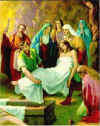
\includegraphics[width=2cm]{jalansalib_files/14_small.jpg}
\end{wrapfigure}
\subsection*{Perhentian XIV\\
YESUS DIMAKAMKAN}

\kamiMenyembah

\BP{Setiap orang pasti mati. Dan kini Tuhan Yesus telah dimakamkan. Dibaringkan dalam sebuah lorong gelap, dingin dan sepi. Ia telah menyelesaikan perutusan-Nya, namun Ia akan bangkit dan membawa keselamatan bagi kita. Penderitaan selalu menyakitkan. Namun terkadang, penderitaan menyimpan suatu rahmat indah di dalamnya. Apakah kita mau untuk selalu setia dalam Tuhan hingga beristirahat bersama-Nya?
\hening
}

\BU{Aku berterima kasih karena Engkau menempuh jalan kami sebagai yang pertama,\\ supaya kamipun boleh beristirahat kelak di rumah Bapa-Mu,\\ dalam diri-Mu dan karena-Mu Terpujilah, Ya Yesus.\\
Tuhan kasihanilah kami (2X)   
}

\large\begin{itemize}\item[~]\it{Bapa Kami - Salam Maria}\end{itemize}\normalsize
\kasihanilahKami

\begin{itemize}
\item[15.] \it{Nama Yesus dimuliakan,\\
	kurban salib dikenangkan,\\
	untuk s’lama lamanya.}
\end{itemize}

\subsection*{Penutup - MERENUNGKAN PASSIO YESUS KRISTUS}

\BP{
Yesus meminta dari kita:

"Renungkanlah bagaimana mereka memperlakukan-Ku dengan keji \dots . Renungkanlah Aku dalam penjara, di mana Aku melewatkan sebagian besar malam itu \dots . Renungkanlah Aku pada malam penuh sengsara ini dan renungkanlah bahwa sengsara ini diperpanjang dalam kesendirian-Ku di begitu banyak Sanctuarium, dalam keacuhan begitu banyak jiwa \dots ."

"Renungkanlah luka-luka-Ku dan lihat apakah ada seorang yang menanggung sengsara sebanyak yang Aku tanggung, demi menunjukkan kasihnya kepadamu \dots . Renungkanlah barang sejenak kedua tangan dan kaki yang bersimbah darah ini \dots . Tubuh telanjang ini, yang penuh luka-luka, dengan urine dan darah. Kotor \dots . Kepala ini, yang ditembusi duri-duri tajam, bermandikan keringat, penuh debu, dan berlumuran darah \dots ."  

"Renungkanlah Yesus-mu, yang tergantung di Salib, tanpa dapat bergerak barang sedikitpun \dots  telanjang, hina, tanpa kehormatan, tanpa kebebasan \dots ."

"Renungkanlah segenap jiwa-jiwa yang akan menelantarkan-Ku di Tabernakel dan banyak jiwa-jiwa yang akan meragukan kehadiran-Ku dalam Ekaristi Kudus \dots ."

"Renungkanlah Aku dalam gambaran Kristus yang berseru dan bersimbah darah. Di sana, dan dengan cara ini, dunia memiliki Aku \dots ."

"Jika engkau sungguh mengasihi Aku, adakah engkau siap untuk menjadi seperti Aku? Apakah yang akan engkau tolak demi taat kepada-Ku, menyenangkan-Ku, menghibur-Ku?..."

"Jiwa-jiwa terkasih, jika kalian tidak menatap Surga, kalian akan hidup sebagai makhluk-makhluk yang tanpa tujuan. Angkatlah kepalamu dan renungkanlah Rumah yang menanti kalian. Carilah Tuhan-mu dan engkau akan senantiasa mendapati-Nya dengan mata-Nya tertuju kepadamu, dan dalam tatapan-Nya engkau akan mendapati damai dan hidup."

	Marilah berdoa,\\
	Allah Mahapengasih, kami bersyukur karena dapat mengenangkan Yesus yang sengsara dan wafat demi keselamatan kami. Limpahkanlah berkat-Mu atas kami yang mengharapkan kebangkitan bersama Dia. Semoga karena berkat-Mu, kami bertumbuh dalam iman dan keyakinan akan kebahagiaan abadi. Demi Kristus Tuhan kami. Amin

Salam Maria \dots $3\times$

Bapa Kami \dots 

Kemulian \dots

Terpujilah \dots
}

\BP{Dalam nama Bapa, dan Putra, dan Roh Kudus. }
\BU{Amin}

\begin{itemize}
\item[~] {\bf Lagu Penutup}
\item[~] Salib di Puncak Kalvari - MB 415
\item[Reff.] \it{
Salib di puncak Kalvari, salib sungguh suci 
}
\item[1.] \it{
Sumber rahmat ilahi, mengalir tanpa henti\\
melimpahkan hidup ilahi, salib sungguh suci
}
\item[2.] \it{
Pohon berbuah cinta, altar tempat berkurban\\
penunjuk jalan yang aman, salib sungguh suci
}
\end{itemize}

\end{document} 

